\documentclass[main]{subfiles}


\title[AutoML: NAS]{Neural Architecture Search}
\subtitle{How to evaluate in Neural Architecture Search?}
\author[Jovita Lukasik]{Jovita Lukasik}
\date{}

\titlebackground*{images/AutoML_NAS}

%\institute{}
%\date{}

\begin{document}
	
	\maketitle

%----------------------------------------------------------------------
\begin{frame}{Motivation}
\begin{itemize}
    \item Evaluating a single architecture requires \alert{full training from scratch} — up to 800 GPU hours for 20k architectures ~\liturl{Zoph and Le 2017}{https://openreview.net/pdf?id=r1Ue8Hcxg}
    \item The \textbf{performance estimation strategy} is the biggest practical bottleneck in NAS
    \item Cheaper estimates allow the search strategy to explore \alert{far more architectures} within the same budget
\end{itemize}
\pause
\vspace{0.5em}
\begin{colorblock}[black]{sintefgrey}{Key Question}
Can we \textbf{reliably predict} which architecture will perform best — without actually training it to convergence?
\end{colorblock}
\end{frame}

\begin{frame}{Definition of Neural Architecture Search}
\begin{center}
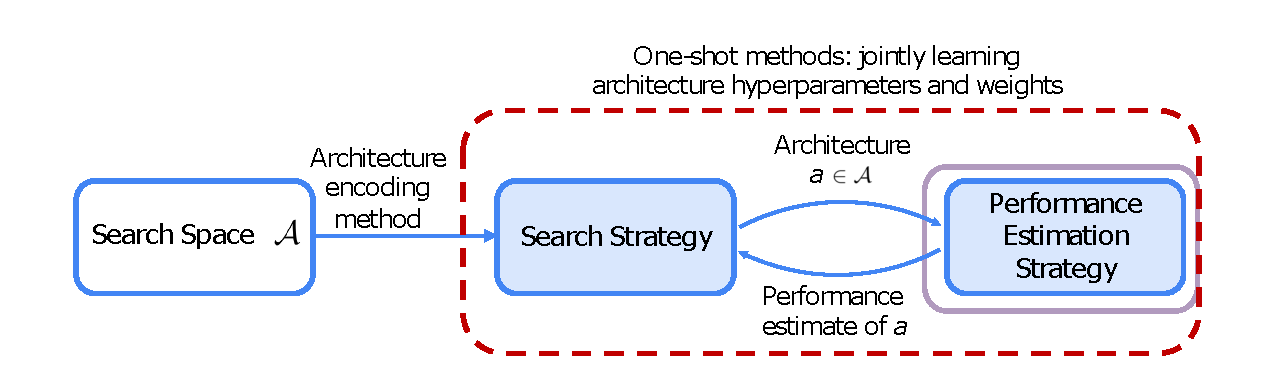
\includegraphics[height=3cm]{images/04/white_2023_nas_overview_3.pdf}
\captionof{figure}{Overview of neural architecture search ~\liturl{White et al. 2023}{https://arxiv.org/pdf/2301.08727.pdf}}
\end{center}
\end{frame}

\begin{frame}{Performance Estimation Strategies}
\begin{itemize}
    \item Evaluation for ground truth accuracy
    \item \alert{Performance prediction methods} (surrogate-based)
  \begin{itemize}
        \item Architecture encoding
        \item Prediction model (Graph Neural Network, Random Forest, MLP, \ldots)
    \end{itemize}
\end{itemize}
\end{frame}



\begin{frame}{Ground Truth}
In the early stages of NAS the architectures were evaluated for their ground truth performance ~\liturl{Zoph and Le 2017}{https://openreview.net/pdf?id=r1Ue8Hcxg}
\begin{itemize}
    \item Up to 20k architectures on CIFAR-10~\liturl{Krizhevsky et al. 2009}{https://www.cs.toronto.edu/~kriz/learning-features-2009-TR.pdf} $\rightarrow$ 800 GPU hours
    \item Since then, the goal is to speed up the evaluation
\end{itemize}
\end{frame}

\begin{frame}{Performance Prediction}
\begin{itemize}
    \item Given a search space $\mathcal{A}$, an architecture $a \in \mathcal{A}$ and the final validation accuracy $\cost(a)$ after full training pipeline $P$
    \item A \textit{performance predictor} $\cost'(a)$ is a function, which predicts the score of the architecture $a$, without $P$. 
    \item Motivation is based on $\cost'(a)$ needing less time for evaluations than $\cost(a)$
    \item Also $\{\cost'(a) \vert a \in A\}$ is ideally highly correlated with  $\{\cost(a) \vert a \in A\}$
\end{itemize}
\end{frame}

\begin{frame}{Performance Predictor - Methods}

% \begin{minipage}{0.5\textwidth}
\begin{itemize}
% \onslide<1-4>
% \item One-shot methods~\liturl{Liu et al. 2019}{https://openreview.net/pdf?id=S1eYHoC5FX}
% \onslide<3-4>
% \begin{enumerate}
    % \item Avoid training each architecture from scratch by one-shot training all architectures in supernetwork
    % \item  Allows for evaluation of each architecture by inheriting weights from supernetwork
% \end{enumerate}
% \onslide<2,4>
\item Surrogate-based methods~\liturl{White et al. 2021}{https://papers.neurips.cc/paper_files/paper/2021/file/ef575e8837d065a1683c022d2077d342-Paper.pdf}
% \onslide<4>
\begin{enumerate}
\item Predict performance of architectures before training them fully
\item Can be combined with different search approaches
\end{enumerate}
\end{itemize}
% $\rightsquigarrow$ We focus here on predictor-based search methods
% \end{minipage}
% \begin{minipage}{0.49\textwidth}
% \onslide<3-4>
% \vspace{-1.5cm}
% 
\includegraphics[width=\textwidth]{07_NAS/images/04/supernet_illustration.pdf}
% \end{minipage}

\end{frame}

\begin{frame}{Performance Predictor Components}


\tikzset{every picture/.style={line width=0.75pt}} %set default line width to 0.75pt        

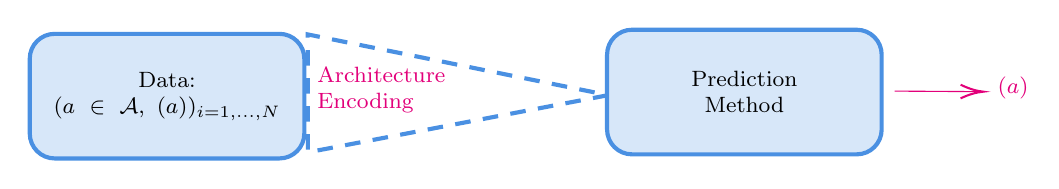
\begin{tikzpicture}[x=0.75pt,y=0.75pt,yscale=-1,xscale=1]
%uncomment if require: \path (0,300); %set diagram left start at 0, and has height of 300

%Shape: Triangle [id:dp3881003956844322] 
\draw  [color={rgb, 255:red, 74; green, 144; blue, 226 }  ,draw opacity=1 ][dash pattern={on 5.63pt off 4.5pt}][line width=1.5]  (298.05,177.51) -- (153.32,205.05) -- (153.23,148.24) -- cycle ;
%Straight Lines [id:da30641777488695965] 
\draw [color={rgb, 255:red, 226; green, 0; blue, 122 }  ,draw opacity=1 ]   (435.97,175.56) -- (453.29,175.67) -- (476.74,175.82) ;
\draw [shift={(478.74,175.84)}, rotate = 180.38] [color={rgb, 255:red, 226; green, 0; blue, 122 }  ,draw opacity=1 ][line width=0.75]    (10.93,-3.29) .. controls (6.95,-1.4) and (3.31,-0.3) .. (0,0) .. controls (3.31,0.3) and (6.95,1.4) .. (10.93,3.29)   ;
%Rounded Rect [id:dp13351727231531285] 
\draw  [color={rgb, 255:red, 74; green, 144; blue, 226 }  ,draw opacity=1 ][fill={rgb, 255:red, 74; green, 144; blue, 226 }  ,fill opacity=0.22 ][line width=1.5]  (19.33,159.97) .. controls (19.33,153.34) and (24.71,147.97) .. (31.34,147.97) -- (139.62,147.97) .. controls (146.25,147.97) and (151.62,153.34) .. (151.62,159.97) -- (151.62,195.99) .. controls (151.62,202.62) and (146.25,208) .. (139.62,208) -- (31.34,208) .. controls (24.71,208) and (19.33,202.62) .. (19.33,195.99) -- cycle ;
%Rounded Rect [id:dp803296283810939] 
\draw  [color={rgb, 255:red, 74; green, 144; blue, 226 }  ,draw opacity=1 ][fill={rgb, 255:red, 74; green, 144; blue, 226 }  ,fill opacity=0.22 ][line width=1.5]  (297.48,158.01) .. controls (297.48,151.38) and (302.86,146) .. (309.49,146) -- (417.77,146) .. controls (424.4,146) and (429.78,151.38) .. (429.78,158.01) -- (429.78,194.03) .. controls (429.78,200.66) and (424.4,206.03) .. (417.77,206.03) -- (309.49,206.03) .. controls (302.86,206.03) and (297.48,200.66) .. (297.48,194.03) -- cycle ;

% Text Node
\draw (363.63,176.02) node  [font=\footnotesize,color={rgb, 255:red, 0; green, 0; blue, 0 }  ,opacity=1 ] [align=left] {\begin{minipage}[lt]{41.27pt}\setlength\topsep{0pt}
\begin{center}
Prediction \\Method
\end{center}

\end{minipage}};
% Text Node
\draw (156.62,162.73) node [anchor=north west][inner sep=0.75pt]  [font=\footnotesize,color={rgb, 255:red, 226; green, 0; blue, 122 }  ,opacity=1 ] [align=left] {Architecture\\ Encoding};
% Text Node
\draw (484.38,167.6) node [anchor=north west][inner sep=0.75pt]  [font=\footnotesize,color={rgb, 255:red, 226; green, 0; blue, 122 }  ,opacity=1 ] [align=left] {$\displaystyle \cost( a)$};
% Text Node
\draw (85.48,177.98) node  [font=\footnotesize] [align=left] {\begin{minipage}[lt]{84.22pt}\setlength\topsep{0pt}
\begin{center}
Data:\\ $\displaystyle ( a\ \in \ \mathcal{A} ,\ \cost( a))_{i=1,...,N}$
\end{center}

\end{minipage}};


\end{tikzpicture}
\captionof{figure}{Overview of performance prediction components}
Performance prediction methods are based on \textbf{three} components:
\begin{itemize}
    \item Dataset to train the prediction method
    \begin{itemize}
        \item Can be also used with learning curve extrapolation
    \end{itemize}
    \item Prediction method for the target $\cost(a)$
    \item Architecture encoding which is the input to the prediction method
\end{itemize}

    % \begin{itemize}
    %     \item \redtodo{todo} train set ... N nets with performance (usually fully trained, but also learning curves/other estimates)
    %     \item predictor -- GNN, RF, XGBoost, ... AutoGluon (used in HW gpt bench (If I don't include it anywhere, Lennart will ask))
    %     \item net encoding -- input to the methods, different variants
    % \end{itemize}
\end{frame}


\begin{frame}{Performance Predictor Components}


\tikzset{every picture/.style={line width=0.75pt}} %set default line width to 0.75pt        

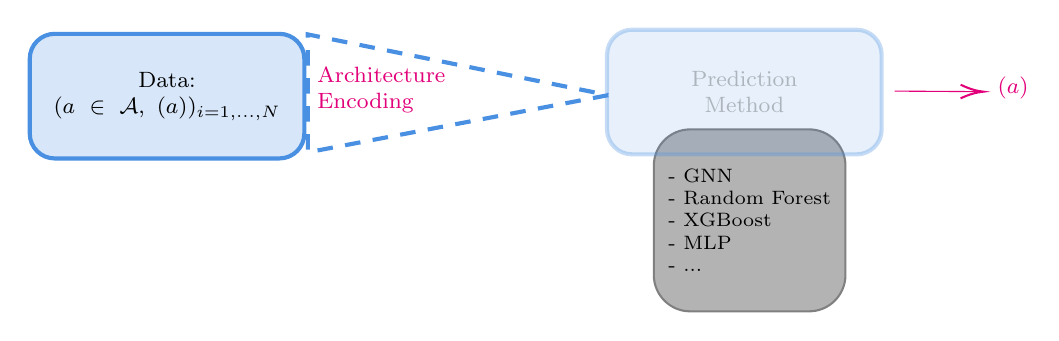
\begin{tikzpicture}[x=0.75pt,y=0.75pt,yscale=-1,xscale=1]
%uncomment if require: \path (0,300); %set diagram left start at 0, and has height of 300

%Rounded Rect [id:dp7559474827809345] 
\draw  [color={rgb, 255:red, 128; green, 128; blue, 128 }  ,draw opacity=1 ][fill={rgb, 255:red, 155; green, 155; blue, 155 }  ,fill opacity=0.76 ][line width=0.75]  (332,113.53) .. controls (332,103.85) and (339.85,96) .. (349.53,96) -- (406.8,96) .. controls (416.48,96) and (424.33,103.85) .. (424.33,113.53) -- (424.33,166.13) .. controls (424.33,175.82) and (416.48,183.67) .. (406.8,183.67) -- (349.53,183.67) .. controls (339.85,183.67) and (332,175.82) .. (332,166.13) -- cycle ;
%Shape: Triangle [id:dp5106397019175131] 
\draw  [color={rgb, 255:red, 74; green, 144; blue, 226 }  ,draw opacity=1 ][dash pattern={on 5.63pt off 4.5pt}][line width=1.5]  (310.05,79.51) -- (165.32,107.05) -- (165.23,50.24) -- cycle ;
%Straight Lines [id:da4265865891852365] 
\draw [color={rgb, 255:red, 226; green, 0; blue, 122 }  ,draw opacity=1 ]   (447.97,77.56) -- (465.29,77.67) -- (488.74,77.82) ;
\draw [shift={(490.74,77.84)}, rotate = 180.38] [color={rgb, 255:red, 226; green, 0; blue, 122 }  ,draw opacity=1 ][line width=0.75]    (10.93,-3.29) .. controls (6.95,-1.4) and (3.31,-0.3) .. (0,0) .. controls (3.31,0.3) and (6.95,1.4) .. (10.93,3.29)   ;
%Rounded Rect [id:dp29720552433048875] 
\draw  [color={rgb, 255:red, 74; green, 144; blue, 226 }  ,draw opacity=1 ][fill={rgb, 255:red, 74; green, 144; blue, 226 }  ,fill opacity=0.22 ][line width=1.5]  (31.33,61.97) .. controls (31.33,55.34) and (36.71,49.97) .. (43.34,49.97) -- (151.62,49.97) .. controls (158.25,49.97) and (163.62,55.34) .. (163.62,61.97) -- (163.62,97.99) .. controls (163.62,104.62) and (158.25,110) .. (151.62,110) -- (43.34,110) .. controls (36.71,110) and (31.33,104.62) .. (31.33,97.99) -- cycle ;
%Rounded Rect [id:dp7719117276092171] 
\draw  [color={rgb, 255:red, 74; green, 144; blue, 226 }  ,draw opacity=0.32 ][fill={rgb, 255:red, 74; green, 144; blue, 226 }  ,fill opacity=0.13 ][line width=1.5]  (309.48,60.01) .. controls (309.48,53.38) and (314.86,48) .. (321.49,48) -- (429.77,48) .. controls (436.4,48) and (441.78,53.38) .. (441.78,60.01) -- (441.78,96.03) .. controls (441.78,102.66) and (436.4,108.03) .. (429.77,108.03) -- (321.49,108.03) .. controls (314.86,108.03) and (309.48,102.66) .. (309.48,96.03) -- cycle ;

% Text Node
\draw (378.17,139.83) node  [font=\scriptsize] [align=left] {\mbox{-} GNN\\\mbox{-} Random Forest\\\mbox{-} XGBoost\\\mbox{-} MLP\\\mbox{-} ...};
% Text Node
\draw (375.63,78.02) node  [font=\footnotesize,color={rgb, 255:red, 0; green, 0; blue, 0 }  ,opacity=0.25 ] [align=left] {\begin{minipage}[lt]{41.27pt}\setlength\topsep{0pt}
\begin{center}
Prediction \\Method
\end{center}

\end{minipage}};
% Text Node
\draw (168.62,64.73) node [anchor=north west][inner sep=0.75pt]  [font=\footnotesize,color={rgb, 255:red, 226; green, 0; blue, 122 }  ,opacity=1 ] [align=left] {Architecture\\ Encoding};
% Text Node
\draw (496.38,69.6) node [anchor=north west][inner sep=0.75pt]  [font=\footnotesize,color={rgb, 255:red, 226; green, 0; blue, 122 }  ,opacity=1 ] [align=left] {$\displaystyle \cost( a)$};
% Text Node
\draw (97.48,79.98) node  [font=\footnotesize] [align=left] {\begin{minipage}[lt]{84.22pt}\setlength\topsep{0pt}
\begin{center}
Data:\\ $\displaystyle ( a\ \in \ \mathcal{A} ,\ \cost( a))_{i=1,...,N}$
\end{center}

\end{minipage}};


\end{tikzpicture}
\captionof{figure}{Overview of performance prediction methods}
The prediction method can be selected from various regression methods in machine learning
Most popular in NAS are: 
% \redtodo{(or some examples are?)}
\begin{itemize}
\item Graph Neural Network
\item Random Forest, XGBoost, MLP
% \item \redtodo{include some bananas}
\end{itemize}
\end{frame}

\begin{frame}{Architecture Encodings}
\begin{columns}
\begin{column}{0.3\textwidth}
    \begin{center}
		
\includegraphics[width=0.3\textwidth, height=2.3
        cm]{07_NAS/images/04/example_graph_encoding.pdf} \\
        {DAG of a neural network cell}
    \end{center}
\end{column}
\begin{column}{0.3\textwidth}
    \begin{center}
        
\includegraphics[width=0.7\textwidth, height=2.3cm]{07_NAS/images/04/example_adj_encoding.pdf} \\
        {Adjacency matrix~\liturl{Yang et al. 2019}{https://arxiv.org/pdf/1902.09635}}
    \end{center}
\end{column}
\begin{column}{0.3\textwidth}
    \begin{center}
	   
\includegraphics[width=0.3\textwidth, height=2.3cm]{07_NAS/images/04/example_path_encodig.pdf} \\
        {Path-based encoding~\liturl{White et al. 2021}{https://cdn.aaai.org/ojs/17233/17233-13-20727-1-2-20210518.pdf}}
    \end{center}
\end{column}
\end{columns}


\begin{itemize}
    \item Circumvent discrete graph representation using different encodings
    \item Facilitate search approaches with performance prediction methods
\end{itemize}
\end{frame}
\iffalse
\begin{frame}{Learning Curve Extrapolation}
\begin{itemize}
    \item Predicts the performance after partial training, by extrapolating from learning curve 
    \item Using parametric model 
    \item Can be combined with surrogate model 
    \item Can be used with black-box NAS
    \item Can be used with multi-fidelity algorithms
\end{itemize}
\end{frame}

\begin{frame}{Zero-Cost Proxies (ZCP)}
    \begin{itemize}
        \item Developed as part of performance prediction \liturl{Mellor et al. 2021}{https://proceedings.mlr.press/v139/mellor21a/mellor21a.pdf}
        \item Run (very) fast computations (one single forward and backward pass on single minibatch of data) over set of architectures to assign a score to each architecture
        \item Hope: score correlated with resulting performance of architecture AFTER full training
        \item Note: ZCP calculated on untrained network! 
        \item Zero-cost since score calculations negligible small
        \item Some ZCP also data-independent, e.g. \# params. 
    \end{itemize}
\end{frame}


\begin{frame}{Performance Prediction Methods in Search}
 Goal in NAS: efficiently find the architecture with the highest validation accuracy for downstream task
\begin{itemize}
    \item Use performance prediction methods to improve search efficiency
    \pause
    \item Predictor-guided evolution: Predictor chooses the next candidates which are evaluated
    \pause
    \item Bayesian optimization + predictor: Ensemble of prediction methods to calculate mean and uncertainty for candidate architectures
\end{itemize}
    % \redtodo{Just one slide about how it's in BO, evo, whatever}

\end{frame}
\fi
%----------------------------------------------------------------------
\begin{frame}{Summary} 

Most important insights from this video:

\begin{enumerate}
    \item Evaluating all architectures from scratch is prohibitively expensive
    \item Performance predictors provide a fast technique for estimating architecture quality
    \item A predictor consists of three components: a dataset of evaluated architectures, an architecture encoding, and a prediction model 
    \item Architecture encoding is a key design choice: adjacency matrices, path encodings, and graph encodings each have different trade-offs
\end{enumerate}


\end{frame}



\end{document}
